\documentclass[10pt]{beamer}
%\usetheme[
%%% option passed to the outer theme
%    progressstyle=fixedCircCnt,   % fixedCircCnt, movingCircCnt (moving is deault)
%]{}
  
% If you want to change the colors of the various elements in the theme, edit and uncomment the following lines

% Change the bar colors:
%\setbeamercolor{Feather}{fg=red!20,bg=red}

% Change the color of the structural elements:
%\setbeamercolor{structure}{fg=red}

% Change the frame title text color:
%\setbeamercolor{frametitle}{fg=blue}

% Change the normal text color background:
%\setbeamercolor{normal text}{fg=black,bg=gray!10}

%-------------------------------------------------------
% INCLUDE PACKAGES
%-------------------------------------------------------

\usepackage[natbib=true,backend=bibtex,useprefix=true]{biblatex}
\addbibresource{bibliography.bib}
\usepackage[utf8]{inputenc}
\usepackage{quoting}
\usepackage{tikz}
\usepackage{ragged2e}
\usepackage{adjustbox}
\justifying

%-------------------------------------------------------
% DEFFINING AND REDEFINING COMMANDS
%-------------------------------------------------------

\usetheme{Warsaw}

%-------------------------------------------------------
% INFORMATION IN THE TITLE PAGE
%-------------------------------------------------------

\title[] % [] is optional - is placed on the bottom of the sidebar on every slide
{ % is placed on the title page
      \textbf{Characterizing and Classifying IoT Traffic in Smart Cities and Campuses}
}

\subtitle[]
{
      \textbf{Paper's analysis\\ITPA 2019-2020}
}

\author[Andrea Graziani - 0273395]
{      Andrea Graziani - 0273395 \\
      {}
}

\institute[]
{
      Università degli Studi di Roma “Tor Vergata” \\
      FACOLTA' DI INGEGNERIA \\
      Corso di Laurea Magistrale in Ingegneria Informatica
  
  %there must be an empty line above this line - otherwise some unwanted space is added between the university and the country (I do not know why;( )
}

\date{\today}

%-------------------------------------------------------
% THE BODY OF THE PRESENTATION
%-------------------------------------------------------

\begin{document}

%-------------------------------------------------------
% THE TITLEPAGE
%-------------------------------------------------------

{% % this is the name of the PDF file for the background
\begin{frame}[plain,noframenumbering] % the plain option removes the header from the title page, noframenumbering removes the numbering of this frame only
  \titlepage % call the title page information from above
\end{frame}}


\section{Introduction}
\subsection{Research's goal}
%---------------------------------------------------------------------------------------------------------%
\begin{frame}{Research's goal}
%---------------------------------------------------------------------------------------------------------%

According to \citet{ITPAReport}, research's goal is to:

\begin{quoting}[font=itshape, begintext={``}, endtext={''}]
[...] develop a classification method that can not only distinguish IoT from non-IoT traffic, but also identify specific IoT devices with over 95\% accuracy.
\end{quoting}

\begin{alertblock}{}
\justifying
What is the reason according to which is important to profile IoT traffic?
\end{alertblock}

\begin{enumerate}
\justifying
\item To understand IoT devices ``\textit{normal}" \textbf{traffic pattern} in terms of their \textbf{activity pattern} (traffic rate, idle durations, etc.) and \textbf{signalling overheads} (\texttt{DNS}, \texttt{NTP}, etc.). 

\item To enhance \textbf{cyber-security} involving IoT devices which administration belong to \textbf{different authorities}. 

According to \citet{ITPAReport}, is possible to improve security deploying a network-level security mechanisms which, analysing traffic patterns, is capable to \textbf{identify attacks knowing the normal traffic pattern of monitored IoT devices}.

\end{enumerate}




%---------------------------------------------------------------------------------------------------------%
\end{frame} 
%---------------------------------------------------------------------------------------------------------%

%---------------------------------------------------------------------------------------------------------%
\begin{frame}{Research's goal}
%---------------------------------------------------------------------------------------------------------%

In other words, research's goal is to build an classification model for IoT devices based on \textbf{machine learning} techniques, which building passes through following steps:

\begin{enumerate}
\item Collect data from an IoT environment.
\item Characterize traffic pattern corresponding to the various IoT devices.
\item Develop a classification technique that learns the behaviour of an IoT device and is able to identify it based on its traffic pattern.
\end{enumerate}







%---------------------------------------------------------------------------------------------------------%
\end{frame} 
%---------------------------------------------------------------------------------------------------------%
\section{IoT Traffic Pattern}
%---------------------------------------------------------------------------------------------------------%
\begin{frame}{Data-set building - Part 1}
%---------------------------------------------------------------------------------------------------------%

\begin{block}{}
\justifying
Since \citet{ITPAReport} adopted a \textbf{supervised machine learning algorithms} to build their classification model, is necessary to generate a \textbf{data-set} in order to provide an appropriate input during the \textbf{learning phase}.
\end{block}

%---------------------------------------------------------------------------------------------------------%
\end{frame} 
%---------------------------------------------------------------------------------------------------------%
%---------------------------------------------------------------------------------------------------------%
\begin{frame}{Data-set building - Part 2}
%---------------------------------------------------------------------------------------------------------%

\begin{itemize}
\justifying
\item \citet{ITPAReport} collected traffic over $3$ weeks generated from a so-called ``\textit{Smart Environment}" built by them. 

\item Is very important to precise that collected data are \textbf{time series}, where each instance, indexed by time, contains several \textbf{attributes} (or \textbf{features}) including:

\begin{itemize}
\item Sleep Time.
\item Active time.
\item Average packet size.
\item peak/mean rate.
\item Number of used protocols.
\item Unique \texttt{DNS} requests. 

\end{itemize}

\item Clearly, every instance contains a \textbf{label} identifying the IoT device, which is necessary during supervised learning.
\end{itemize}


%---------------------------------------------------------------------------------------------------------%
\end{frame} 
%---------------------------------------------------------------------------------------------------------%
\subsection{The ``Smart Environment"}
%---------------------------------------------------------------------------------------------------------%
\begin{frame}{The ``Smart Environment" - Part 1}
%---------------------------------------------------------------------------------------------------------%

\begin{itemize}
\justifying
\item In order to build the necessary dataset, \citet{ITPAReport} built the aforementioned ``\textit{Smart Environment}" to simulate a real usage scenario, collecting required data.

\item This environment is made up of:

\begin{itemize}
\justifying
\item $21$ unique IoT devices representing different categories, like \textbf{cameras}, \textbf{healthcare devices}, \textbf{hub}, \textbf{air quality sensors} and so on.

\item A router, the \textsc{TP Link Archer C7}\footnote{\tiny\url{https://www.tp-link.com/it/home-networking/wifi-router/archer-c7/\#overview}}

\item Several non-IoT devices were also used, such as laptops, mobile phones and tablet.

\end{itemize}
\end{itemize}

\begin{figure}
  \caption{``Smart environment"'s scheme}
  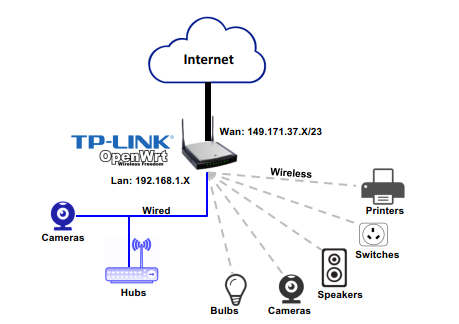
\includegraphics[width=100pt]{Topology.png}
\end{figure}

%---------------------------------------------------------------------------------------------------------%
\end{frame} 
%---------------------------------------------------------------------------------------------------------%
%---------------------------------------------------------------------------------------------------------%
\begin{frame}{The ``Smart Environment" - Part 2}
%---------------------------------------------------------------------------------------------------------%

\begin{block}{}
Several IoT devices used by \citet{ITPAReport} for their experiments \textbf{are battery operated}. 

For instance:

\begin{itemize}
\justifying
\item The \textit{Withings Smart scale} device is powered by $4$ $1.5$ \textit{V} alkaline cells (AAA).\footnote{\url{https://www.withings.com/it/en/body}}

\item Similarly, the \textit{Netatmo Weather station} device is powered by $2$ $1.5$ \textit{V} alkaline cells (AAA) with an \textbf{estimated autonomy of about 2 years}.\footnote{\url{https://www.netatmo.com/it-it/weather/weatherstation/specifications}
}
\item The \textit{Blipcare blood pressure meter} device is powered by an internal battery.\footnote{\url{http://www.blipcare.com/}}
\end{itemize} 

\end{block}

%---------------------------------------------------------------------------------------------------------%
\end{frame} 
%---------------------------------------------------------------------------------------------------------%
\subsection{``Smart Environment" Architecture}
%---------------------------------------------------------------------------------------------------------%
\begin{frame}{``Smart Environment" Architecture - Part 1}
%---------------------------------------------------------------------------------------------------------%

The architecture of the ``Smart Environment"  can be splitted into:

\begin{description}
\justifying
\item[\textbf{Front-end}] which contains the \textit{router} and the \textit{IoT/non-IoT devices}

\item[\textbf{Back-end}] represented by the \textit{cloud} which is responsible for computations, storing received information, filtering duplicate packets and so on.
through the gateway

\end{description}

\begin{block}{}
\justifying
Cloud resources are exploited through so-called \textbf{cyber-foraging techniques} in order to overcome the very strictly constrains of any IoT devices.
\end{block}

\begin{block}{}
\justifying
Proposed architecture is intended for \textbf{cloud-native} applications.
\end{block}

%---------------------------------------------------------------------------------------------------------%
\end{frame} 
%---------------------------------------------------------------------------------------------------------%
%---------------------------------------------------------------------------------------------------------%
\begin{frame}{``Smart Environment" Architecture - Part 2}
%---------------------------------------------------------------------------------------------------------%

\begin{block}{}
The front-end of the ``Smart Environment", build by researchers, is characterized by a \textbf{star network topology}.
\end{block}

This is a very important observation, because a star topology allows us to:

\begin{itemize}
\justifying
\item \textbf{Preserve battery life} of IoT devices because they \textbf{do not have to forward} other nodes data; in other words, \textit{any IoT device receives, or transmits, only its own data}.

\item \textbf{Decrease the complexity} of the network.
\end{itemize}

\begin{block}{The LPWAN example}
\justifying
The implementation of \texttt{LoRaWAN} network is based on the star network topology, and mostly, stars-of-stars network. 

As known \texttt{LoRaWAN} network belongs to \texttt{LPWAN} category, \textit{which are specifically designed to achieve the need for low power, long-range, low bit error rate, and low cost} needed in IoT context. 
\end{block}

%---------------------------------------------------------------------------------------------------------%
\end{frame} 
%---------------------------------------------------------------------------------------------------------%
\subsection{``Smart Environment"'s Wireless Networks Technology}
%---------------------------------------------------------------------------------------------------------%
\begin{frame}{``Smart Environment"'s Wireless Networks Technology}
%---------------------------------------------------------------------------------------------------------%

According to vendor's specifications regarding the \textsc{TP Link Archer C7}, is possible to know that the aforementioned router supports following protocols:

\begin{itemize}
\item \texttt{IEEE 802.11ac/n/a} at $5$ GHz
\item \texttt{IEEE 802.11n/b/g} at $2.4$ GHz
\end{itemize}

\begin{block}{}
Researchers use \texttt{IEEE 802.11} as \textbf{media access control} (\texttt{MAC}) and \textbf{physical layer} (\texttt{PHY}) protocol.
\end{block}

\begin{block}{}
Researchers did \textit{not} specify which \textbf{version} of IEEE 802.11 standard has been effectively used. 

We don't know with which \textbf{frequencies} data has been transmitted.
\end{block}

%---------------------------------------------------------------------------------------------------------%
\end{frame} 
%---------------------------------------------------------------------------------------------------------%
%---------------------------------------------------------------------------------------------------------%
\begin{frame}{``Smart Environment"'s Wireless Networks Technology}
%---------------------------------------------------------------------------------------------------------%

\begin{block}{}
\justifying
We believe that above protocols are \textbf{not} fully optimized for IoT business models and devices used in smart cities and campuses for following reasons:

\begin{itemize}
\justifying
\item These technologies provide a \textbf{short/medium coverage} with \textbf{100-to-1000} meters range. Provided coverage range can be not enough to fulfil all use cases.

\begin{itemize}
\item This is due to \textbf{mid/high frequencies} used by these protocol which are \textbf{vulnerable to several side effect during signal propagation} (\textit{blocking}, \textit{reflection}, \textit{refraction} and so on)
\end{itemize}

\item They are affected by \textbf{header-overhead} caused by \textbf{short packets transmission} which are very common is many IoT scenarios.

\end{itemize}
\end{block}


%---------------------------------------------------------------------------------------------------------%
\end{frame} 
%---------------------------------------------------------------------------------------------------------%
%---------------------------------------------------------------------------------------------------------%
\begin{frame}{``Smart Environment"'s Wireless Networks Technology}
%---------------------------------------------------------------------------------------------------------%

\begin{block}{}
\justifying
Utilizing sub-1 GHz bands used by both \texttt{802.11ah} and \texttt{LoRaWAN}, is possible to provide \textbf{better  propagation characteristics} in outdoor scenarios. 

\textbf{Low frequencies signal are less affected by obstacles presence.}
\end{block}

\begin{block}{}
A combination of low-band, mid-band and high-band spectrum is desirable to manage all possible use cases.
\end{block}

\begin{adjustbox}{width=\columnwidth,center}
\begin{tabular}{l|ccccc}

& \textbf{802.11ac} & \textbf{802.11n} & \textbf{802.11a} & \textbf{802.11ah} & \textbf{LoRaWAN} \\
\hline
\textbf{Frequency (GHz)} & $5$ & $2.4$,$5$ & $5$ & $0.7/0.8/0.9$ & $\backsim 0.86 (EU)$ \\
\textbf{Sensitivity (dbm)} & $-82$ & $-82$ & $-88$ & $-98$ &  $[-124,-137]$ \\
\textbf{Bit rate} & $6.5$ (Mb/s) & $6.5$ (Mb/s) & $1.5$ (Mb/s) & $0.15$ (Mb/s) & $5469$ (Bit/s) \\
\textbf{Max coverage range (km)} & $0.115$ & $0.230$ & $0.115$ & $\backsim 1$ & $\backsim 15$ \\

\end{tabular}
\end{adjustbox}


%---------------------------------------------------------------------------------------------------------%
\end{frame} 
%---------------------------------------------------------------------------------------------------------%
\subsection{IoT Traffic}
%---------------------------------------------------------------------------------------------------------%
\begin{frame}{IoT Traffic - Part 1}
%---------------------------------------------------------------------------------------------------------%

According to their experimental results, \citet{ITPAReport} stated that:

\begin{quoting}[font=itshape, begintext={``}, endtext={''\cite[par.~IV.A]{ITPAReport}}]
\justifying
[...] if we consider only the load imposed by the IoT devices, then there is a dramatic reduction in the peak load ($1$ Mbps) and average loads ($66$ Kbps), [...], implying that traffic generated by IoT devices is small compared to traditional non-IoT traffic. 
\end{quoting}

\begin{quoting}[font=itshape, begintext={``}, endtext={''\cite[par.~IV.A]{ITPAReport}}]
\justifying
the traffic pattern of one IoT device [...] a pattern of active/sleep communication emerges. [...] IoT active time [...] decays rapidly initially (only 5\% of sessions last longer than 5 seconds), with the maximum active time being 250 seconds in our trace. This shows that IoT activities are short-lived in general. 
\end{quoting}

%---------------------------------------------------------------------------------------------------------%
\end{frame} 
%---------------------------------------------------------------------------------------------------------%
%---------------------------------------------------------------------------------------------------------%
\begin{frame}{IoT Traffic - Part 2}
%---------------------------------------------------------------------------------------------------------%

\begin{block}{}
\justifying
Since many IoT devices are battery powered, \textbf{maximize energy efficiency}, in order to \textbf{preserve devices lifetime}, is critical. 
\end{block}

\begin{block}{}
\justifying
According to \citet{ITPAReport}'s results, the power management approach adopted by IoT devices is based on \textbf{periodic sleep}, during which radio transceiver are turned off.
\end{block}

\begin{figure}
  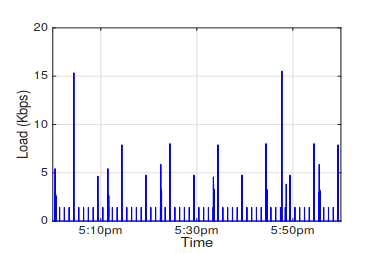
\includegraphics[width=150pt, height=80pt]{SleepTime.png}
  \caption{Load of LiFX light bulb device.}
  \label{fig1}
\end{figure}

%---------------------------------------------------------------------------------------------------------%
\end{frame} 
%---------------------------------------------------------------------------------------------------------%
%---------------------------------------------------------------------------------------------------------%
\begin{frame}{IoT Traffic - Part 3}
%---------------------------------------------------------------------------------------------------------%

\begin{itemize}
\justifying
\item A very interesting observation by \citet{ITPAReport} made by regard packet size, according to which only the $10\%$ of packets are larger than $500$ Bytes.

\begin{itemize}
\item \textbf{header-overhead}, caused by \textbf{short packets transmission}, can occur frequently.
\end{itemize}

\end{itemize}

\begin{figure}
  \caption{``Smart environment"'s scheme}
  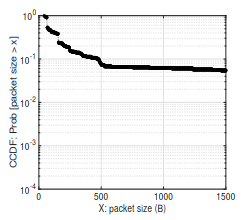
\includegraphics[width=100pt]{PacketSize.png}
\end{figure}

%---------------------------------------------------------------------------------------------------------%
\end{frame} 
%---------------------------------------------------------------------------------------------------------%


%---------------------------------------------------------------------------------------------------------%
\begin{frame}{IoT Application Layer Protocol: Overview}
%---------------------------------------------------------------------------------------------------------%

\begin{itemize}

\item According to \cite{REALSMARTIOT}, smart city and campus services services are based on a
centralized architecture where a dense and heterogeneous set of IoT devices generate differ-
ent types of data that are then delivered through suitable com-
munication technologies to a control center, where data storage
and processing are performed

peripheral devices deployed over the urban area generate differ-
ent types of data that are then delivered through suitable com-
munication technologies to a control center, where data storage
and processing are performed




\item A very important aspect is the necessity to make
(part of) the data collected by the urban IoT easily accessible
by authorities and citizens,

\end{itemize}




%---------------------------------------------------------------------------------------------------------%
\end{frame} 
%---------------------------------------------------------------------------------------------------------%
\section{IoT Application Layer Protocols}
\subsection{The Most Dominant Application Layer Protocols}
%---------------------------------------------------------------------------------------------------------%
\begin{frame}{The Most Dominant Application Layer Protocols - Part 1}
%---------------------------------------------------------------------------------------------------------%

\begin{figure}
  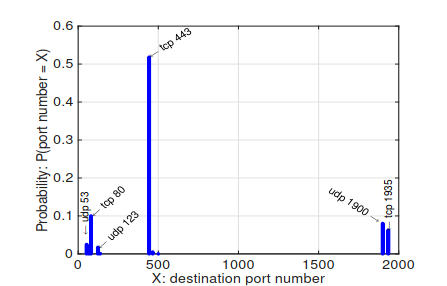
\includegraphics[width=250pt]{PacketType.png}
  \caption{Probability histogram of destination port numbers for IoT packets destined to both the local network and the Internet.}
\end{figure}

%---------------------------------------------------------------------------------------------------------%
\end{frame} 
%---------------------------------------------------------------------------------------------------------%
%---------------------------------------------------------------------------------------------------------%
\begin{frame}{The Most Dominant Application Layer Protocols - Part 2}
%---------------------------------------------------------------------------------------------------------%

\begin{description}
\justifying

\item[\texttt{HTTPS}] (\texttt{TCP} port $443$) is the dominant protocol used by the IoT devices since it represents over the $55\%$ of total IoT traffic.

\item[\texttt{HTTP}] (\texttt{TCP} port $80$) represent the second most dominant application layer protocol constituting the $11\%$ of total traffic.

\item[\texttt{SSDP}] (\texttt{UDP} port $1900$) is the next most dominant application layer protocol representing the $8\%$ of traffic.

\begin{itemize}
\item SSDP, which stands for \textbf{Simple Service Discovery Protocol}, is used to for \textit{advertisement} and \textit{discovery} purposes of network services without the assistance of server-based configuration mechanisms, such as \texttt{DHCP} or \texttt{DNS}.
\end{itemize}

\item[\texttt{RTMP}] (\texttt{TCP} port $1935$) represent the fourth most dominant protocol representing the $7\%$ of traffic

\begin{itemize}
\item \texttt{RTMP}, which stands for \textbf{Real-Time Messaging Protocol}, is a proprietary protocol used for streaming audio, video and data over the Internet, generally used by cameras. It is owned by Adobe.
\end{itemize}

\end{description}

%---------------------------------------------------------------------------------------------------------%
\end{frame} 
%---------------------------------------------------------------------------------------------------------%
%---------------------------------------------------------------------------------------------------------%
\begin{frame}{The Most Dominant Application Layer Protocols - Part 3}
%---------------------------------------------------------------------------------------------------------%

\begin{description}
\justifying
\item[\texttt{DNS}] (\texttt{UDP} port $53$) represents less than $5/4\%$ of total traffic.

\item[\texttt{NTP}] (\texttt{UDP} port $123$) constitutes less than $2/3\%$ of IoT traffic.

\item[Application specific] \citet{ITPAReport}'s results shows that, regarding remaining IoT traffic, each IoT device use an own \textbf{application-specific} protocol. 

In table reported below, are reported most frequent \textit{transportation protocol} and \textit{port number}.

\begin{figure}
  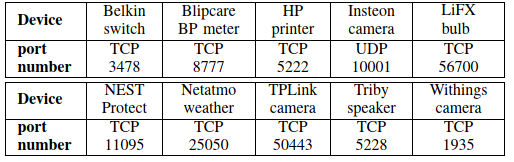
\includegraphics[width=250pt]{port.png}
\end{figure}

\end{description}

%---------------------------------------------------------------------------------------------------------%
\end{frame} 
%---------------------------------------------------------------------------------------------------------%
\subsection{The role of \texttt{HTTP}}
%---------------------------------------------------------------------------------------------------------%
\begin{frame}{The role of \texttt{HTTP} - Part 1}
%---------------------------------------------------------------------------------------------------------%

\begin{alertblock}{}
\textit{Why results that \texttt{HTTPS} and \texttt{HTTP} are the most used protocols by IoT devices?}
\end{alertblock}

\begin{itemize}
\justifying
\item A very important aspect of an urban, or campus, IoT infrastructure is the \textbf{necessity to make data collected by the urban IoT devices easily accessible} by both authorities and citizens.

\item In order to achieve this objective, IoT devices adopt a very well known web-based paradigm called  \textbf{Representational State Transfer} (\textbf{ReST}), which plays a very important role into \textbf{Web of Things Architecture} (\textbf{WoT}).

\end{itemize}


%---------------------------------------------------------------------------------------------------------%
\end{frame} 
%---------------------------------------------------------------------------------------------------------%
%---------------------------------------------------------------------------------------------------------%
\begin{frame}{The role of \texttt{HTTP} - Part 2}
%---------------------------------------------------------------------------------------------------------%

\begin{itemize}
\justifying
\item Exploiting REST paradigm, \texttt{HTTP} and \texttt{HTTPS} are used very frequently because they facilitate both the \textbf{integration of IoT devices} with existing services currently available on the Web and the  \textbf{Web applications development}.

\item \texttt{HTTP} and \texttt{HTTPS} offer a \textbf{direct access} for users to IoT devices data and services, without the need for installing additional software. 

In fact, using a Web browser (or any \texttt{HTTP} library in the case of a software client) client are able to to directly extract, save and share smart things data and services. 

\textbf{This ensures the usability of the architecture and minimizes the entry barriers for final users.}
\end{itemize}

%---------------------------------------------------------------------------------------------------------%
\end{frame} 
%---------------------------------------------------------------------------------------------------------%
\subsection{The disadvantages of \texttt{HTTP}}
%---------------------------------------------------------------------------------------------------------%
\begin{frame}{The disadvantages of \texttt{HTTP}}
%---------------------------------------------------------------------------------------------------------%

\begin{itemize}
\justifying
\item The \textbf{verbosity} and \textbf{complexity} of native \texttt{HTTPS}/\texttt{HTTP} make them \textbf{unsuitable} for constrained IoT devices. 

\begin{itemize}
\justifying
\item In fact, the \textbf{human-readable format} of \texttt{HTTP}, which has been one of the reasons of its success in traditional networks, turns out to be a limiting factor due to the large amount of heavily correlated (and, hence, \textbf{redundant}) data.
\end{itemize}

\item \texttt{HTTPS}/\texttt{HTTP} rely upon the \texttt{TCP} transport protocol that, however, does not scale well on constrained devices, yielding poor performance for small data flows in lossy environments.
\end{itemize}

%---------------------------------------------------------------------------------------------------------%
\end{frame} 
%---------------------------------------------------------------------------------------------------------%
\subsection{An Unbalanced Data-Set}
%---------------------------------------------------------------------------------------------------------%
\begin{frame}{An Unbalanced Data-Set - Part 1}
%---------------------------------------------------------------------------------------------------------%

\begin{block}{}
\justifying
The performance and the interpretation of a IoT device classification model \textbf{depend heavily on the data} on which it was \textbf{trained}. 

\begin{itemize}
\justifying
\item Scientific literature showed that classification model, which are trained on \textit{imbalanced datasets}, are highly susceptible to producing inaccurate results. 
\end{itemize}
\end{block}

\begin{block}{}
The dataset produced by researchers can be unbalanced owing to several reasons including:

\begin{itemize}
\item Too few IoT device types.
\item \textit{Constrained} and \textit{unconstrained} protocol stack are not equally represented into dataset.
\end{itemize}

\end{block}

%---------------------------------------------------------------------------------------------------------%
\end{frame} 
%---------------------------------------------------------------------------------------------------------%
%---------------------------------------------------------------------------------------------------------%
\begin{frame}{An Unbalanced Data-Set - Part 2}
%---------------------------------------------------------------------------------------------------------%

\begin{itemize}
\justifying
\item Generally smart city and campus services are based on a \textbf{very heterogeneous set of IoT devices}, generating \textbf{very different types of data} that have to be delivered through \textbf{suitable communication technologies}.

\item For instance, possible applications can be:

\begin{itemize}
\item Structural Health of Buildings.
\item Waste Management.
\item Air Quality.
\item Traffic Congestion.
\item Noise Monitoring.
\item City Energy Consumption.
\item Smart Parking.
\item Smart Lighting.
\end{itemize}

\end{itemize}

\begin{block}{}
Proposed ``\textit{Smart environment}" seem to be more suitable for a smart home rather than a smart city or campus.
\end{block}

%---------------------------------------------------------------------------------------------------------%
\end{frame} 
%---------------------------------------------------------------------------------------------------------%
%---------------------------------------------------------------------------------------------------------%
\begin{frame}{An Unbalanced Data-Set - Part 3}
%---------------------------------------------------------------------------------------------------------%

\begin{block}{}
\justifying

The ``\textit{Smart environment}" used by researchers \textit{can} be \textit{not} suitable for their purposes because is \textbf{too simple}.

\begin{itemize}
\justifying

\item It includes \textbf{only} \textit{unconstrained protocol stack} which include protocols that are currently the de-facto standards for Internet communications and are commonly used by regular Internet hosts (\texttt{HTTP}/\texttt{TCP}/\texttt{IPv4}).

\begin{itemize}
\justifying
\item In fact there is a prevalence of \texttt{HTTPS}/\texttt{HTTP} application layer protocol ($66\%$ of total IoT traffic according to \citet{ITPAReport}) and of the \texttt{TCP} transport layer protocol (representing, more or less, the $85\%$ of total transmitted packets according to \citet{ITPAReport}'s results).
\end{itemize}

\item It does \textbf{not} include any \textit{constrained protocol stack}, the low-complexity counterparts of the de-facto standards for Internet, i.e., \textbf{Constrained Application Protocol} (\texttt{CoAP}), \texttt{UDP}, and \texttt{6LoWPAN}, which are suitable even for very constrained devices.

\end{itemize}

\end{block}


%---------------------------------------------------------------------------------------------------------%
\end{frame} 
%---------------------------------------------------------------------------------------------------------%
\subsection{Differences between IoT and Non-IoT Traffic}
%---------------------------------------------------------------------------------------------------------%
\begin{frame}{Differences between IoT and Non-IoT Traffic}
%---------------------------------------------------------------------------------------------------------%

Experiment's results show following differences among IoT and Non-IoT traffic:

\begin{description}
\item[DNS traffic] IoT devices initiate DNS queries for only a limited number of domains while non-IoT device, such as a laptop, looks for more than $300$ domain names in a course of a few hours.

\item[Number of Cloud servers] IoT device communicates with less than $10$ servers on average per day while non-IoT device contacts about $500$ different servers
\end{description}


%---------------------------------------------------------------------------------------------------------%
\end{frame} 
%---------------------------------------------------------------------------------------------------------%
\subsection{Security Problems Due To Unencrypted Traffic}
%---------------------------------------------------------------------------------------------------------%
\begin{frame}{Security Problems Due To Unencrypted Traffic - Part 1}
%---------------------------------------------------------------------------------------------------------%

\begin{alertblock}{}
\textit{IoT devices communication is properly secured?}
\end{alertblock}

\begin{itemize}
\justifying

\item According to \citet{ITPAReport}, about $45\%$ of IoT traffic is not sent over HTTPS to the servers. 

\item Since the traffic transmitted using other protocols are typically not encrypted, \citet{ITPAReport}'s results indicate that a sizeable fraction of IoT traffic is \textbf{not} being securely transported over the Internet.

\begin{itemize}
\item The use of unencrypted protocols can leak sensitive information about users.
\end{itemize}

\end{itemize}


%---------------------------------------------------------------------------------------------------------%
\end{frame} 
%---------------------------------------------------------------------------------------------------------%
%---------------------------------------------------------------------------------------------------------%
\begin{frame}{Security Problems Due To Unencrypted Traffic - Part 2}
%---------------------------------------------------------------------------------------------------------%

\begin{alertblock}{}
\textit{Why IoT devices transmit unencrypted data?}
\end{alertblock}

There may be various reasons according to which data are transmitted unencrypted:

\begin{itemize}
\justifying

\item Due to \textbf{limitations} and \textbf{constrains} in the IoT device itself. 

\item As noted by Englehardt and Narayanan [25], IoT devices vendors may be hesitant to move to \texttt{HTTPS} if their products use any third-party resources that are \texttt{HTTP}-only. These resources are typically ads and trackers.

\item Bad design.

\end{itemize}


%---------------------------------------------------------------------------------------------------------%
\end{frame} 
%---------------------------------------------------------------------------------------------------------%
%---------------------------------------------------------------------------------------------------------%
\begin{frame}{}
%---------------------------------------------------------------------------------------------------------%







available technologies. From the table, it clearly
emerges that, in general, the practical realization of most
of such services is not hindered by technical issues, but rather
by the lack of a widely accepted communication and service
architecture that can abstract from the specific features of the
single technologies and provide harmonized access to the
services.

\begin{itemize}
\item According to \citet{ITPAReport}, the set of IoT devices used for their experiments including a huge amount of \textbf{sensors}, including air quality sensors and health-care devices. 

As known, aforementioned kind of devices generate a huge amount of data modelled as \textbf{time series}, that is an array of values indexed by time. 

According to \citet{TIMESERIES}, the stream of data generated by all these IoT sensors is generally interfaced with database, through a so-called \textit{southbound} interface, using HTTP RESTful protocol. Similarly, all applications requiring access to the data stored in the database, using the same protocol, through a so-called northbound interface. 

\end{itemize}
%---------------------------------------------------------------------------------------------------------%
\end{frame} 
%---------------------------------------------------------------------------------------------------------%









\begin{frame}[noframenumbering,shrink=15]{Some references}
\printbibliography
\end{frame}
\end{document}
